\section{Runtime View}
In this section the run-time view of our system will be described with respect to its main functionalities. We mainly focused our attention on critical aspects such as the creation of a new task and the management of shared based vehicles.

\subsection{Sign up and Log in}
The sign up process is not a critical one but we have decided to include its description since it involves all the main layers of our application. 
The process starts with the Client sending a sign up request, which is made up of a mail and password to the Application Façade; this request is then packed in a HTTPS message and sent to the Presenter which is in charge of parsing the message and dispatch it to the Business Logic. At this point the data received will be checked and if everything its okey a new user will be registered and a confirmation mail will be sent to the corresponding email, otherwise an error message will be sent to the Client passing through the Presenter and the Application Façade.
The same is valid for the Log in process but in such a case if the data are correct then the Client will be validated and logged into the system.

\begin{figure}[H]
    \centering
    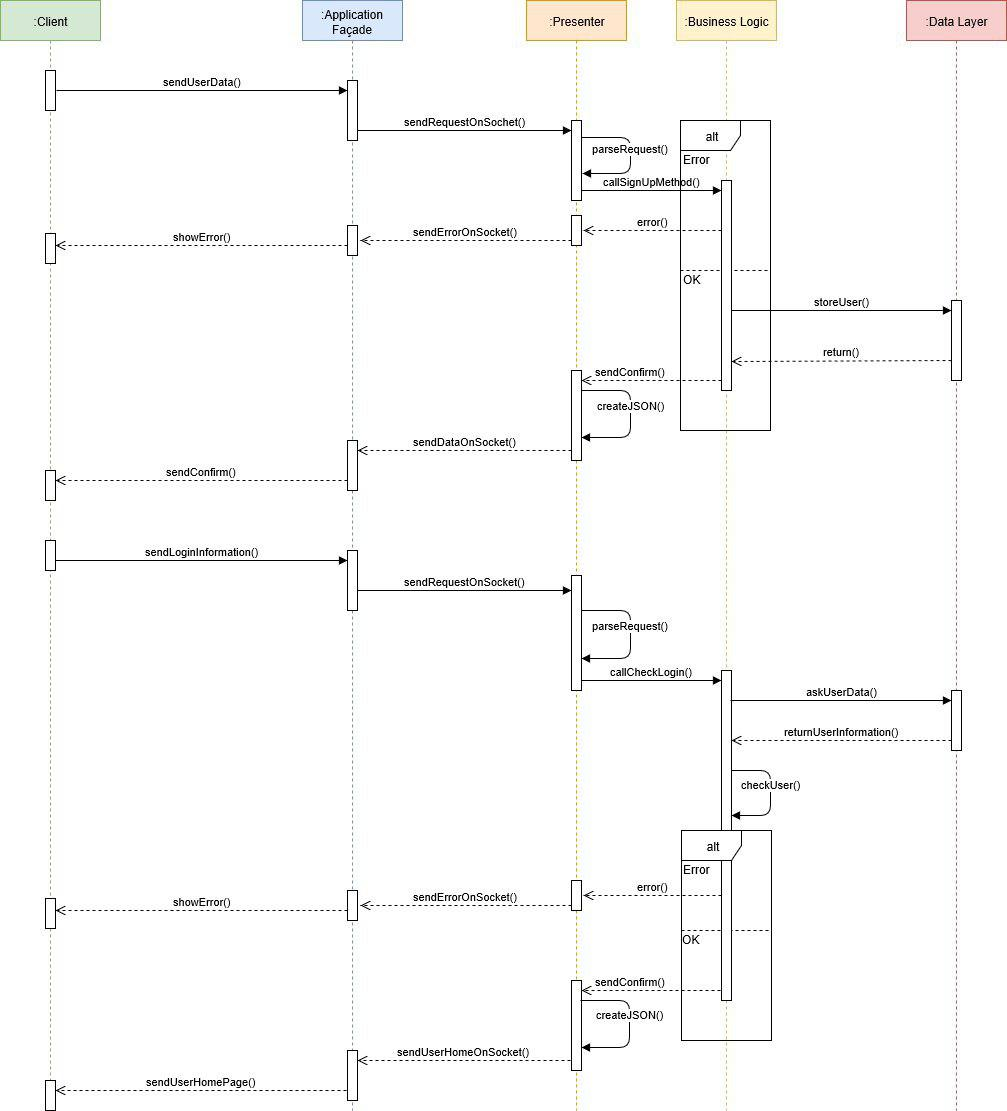
\includegraphics[scale=0.55]{Pictures/RunTimeView/signIn.jpg}
    \caption{Sequence Diagram for the Sign up of a new User}
    \label{fig:sequenceSignUp}
\end{figure}

\subsection{Add a Task}
The creation of a new Task starts with the Client sending all the information required for the creation of a new Task (see \textcolor{red}{Task entity}) to the Application Façade. This information will be properly packed in an HTTPS message and sent to the Presenter. At this point the message will be parsed and dispatched to the Business Logic component in charge for the Business work flow; now the system will try to schedule the newly inserted task in the calendar (loaded from the Database) and if no conflicts occur, then the new schedule will be sent to the user through the Presenter and the Application Façade. If the calendar is approved by the client then it will be stored in the Database.
Notice that a very similar process is performed when the Client require to modify a task preference or wants to remove a task. 

\begin{figure}[H]
    \centering
    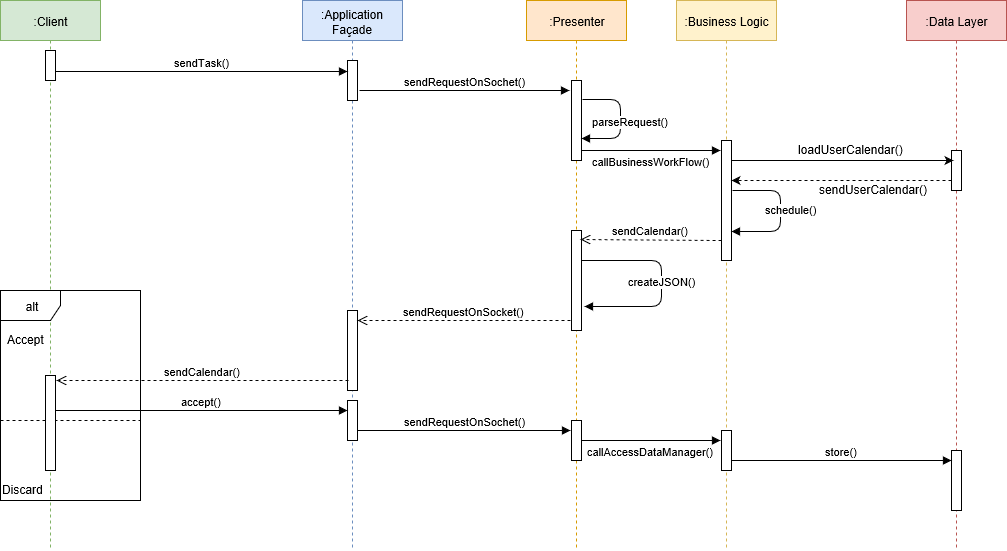
\includegraphics[scale=0.4]{Pictures/RunTimeView/addTask.png}
    \caption{Sequence Diagram for the creation of a new task}
    \label{fig:sequenceAddTask}
\end{figure}

\subsection{Reminder}
The usage of every kind of shared based vehicle is supported by a reminder system, as previously detailed in the \emph{RASD Document} of the project. For this reason a component of the Business Logic will be in charge to ask the calendar of every user to the Data Layer and then check the availability of such vehicles 30 minutes before the travel starts. If there are vehicles available within the maximum walk range, then the user will be notified of the closest one; otherwise a reschedule of the day will occur and the user will be notified of the potential changes. 


\begin{figure}[H]
    \centering
    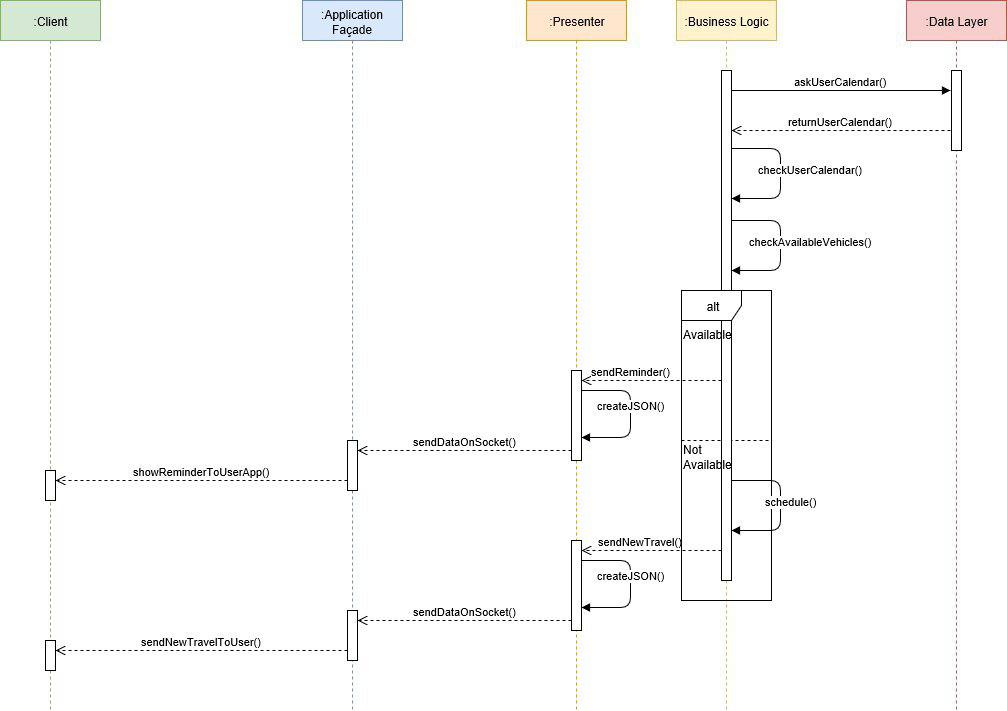
\includegraphics[scale=0.55]{Pictures/RunTimeView/reminder.jpg}
    \caption{Sequence Diagram for checking availability of shared based vehicles}
    \label{fig:sequenceReminder}
\end{figure}